\documentclass[border=2pt]{standalone}
\usepackage{tikz}
\usetikzlibrary{shapes.geometric, arrows.meta, positioning, calc}
\usepackage{xcolor}

% Style Guide Colors
\definecolor{Garnet}{HTML}{73000A}
\definecolor{Gray10}{gray}{0.10}
\definecolor{Gray30}{gray}{0.30}
\definecolor{Gray50}{gray}{0.50}
\definecolor{Gray70}{gray}{0.70}
\definecolor{Gray90}{gray}{0.90}

\begin{document}

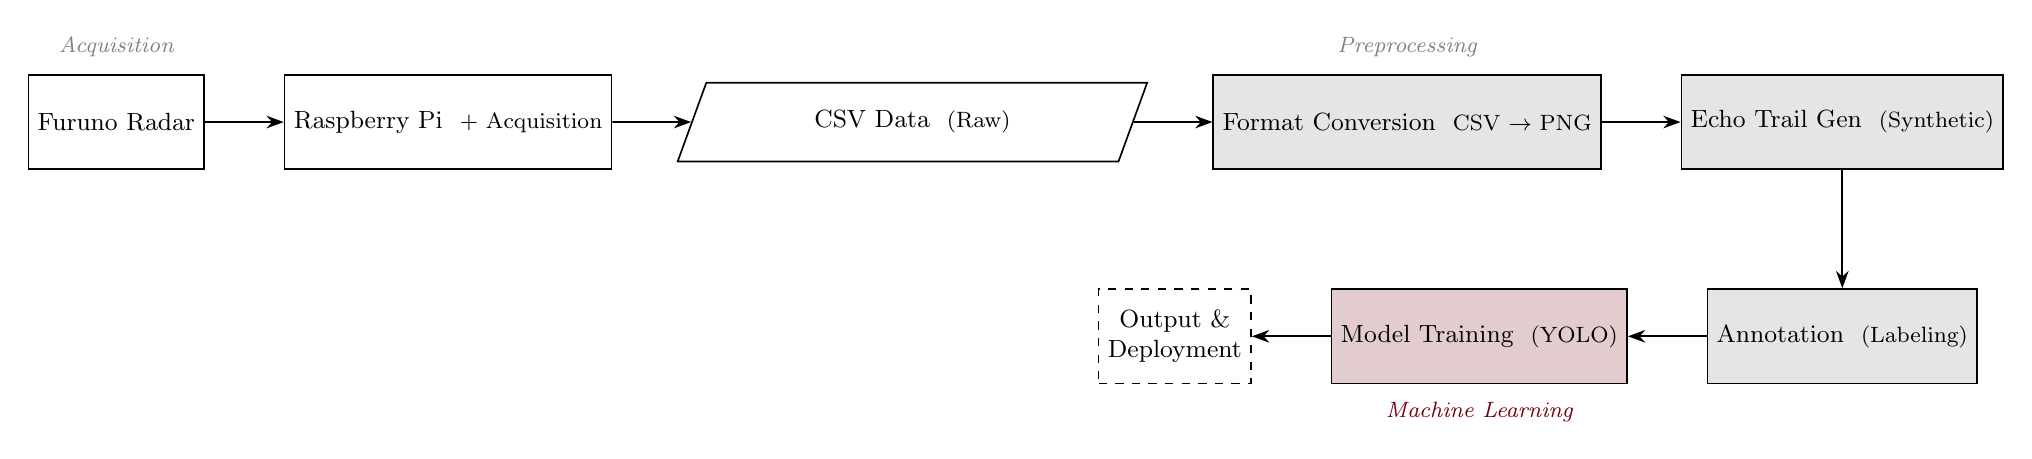
\begin{tikzpicture}[
    % Global Styles
    node distance=1.5cm and 1.0cm,
    font=\small,
    % Styles for different component types
    hardware/.style={
        rectangle, 
        draw=black, 
        fill=white, 
        line width=0.6pt,
        minimum height=1.2cm, 
        minimum width=1cm, 
        align=center
    },
    process/.style={
        rectangle, 
        draw=black, 
        fill=Gray90, 
        line width=0.6pt,
        minimum height=1.2cm, 
        minimum width=1cm, 
        align=center
    },
    data/.style={
        trapezium, 
        trapezium left angle=70, 
        trapezium right angle=110, 
        draw=black, 
        fill=white, 
        line width=0.6pt,
        minimum height=1.0cm, 
        minimum width=1cm, 
        align=center
    },
    ml/.style={
        rectangle, 
        draw=black, 
        fill=Garnet!20, % Light garnet tint for emphasis
        line width=0.6pt,
        minimum height=1.2cm, 
        minimum width=1cm, 
        align=center
    },
    deployment/.style={
        rectangle, 
        draw=black, 
        dashed,
        fill=white, 
        line width=0.6pt,
        minimum height=1.2cm, 
        minimum width=1cm, 
        align=center
    },
    % Connector line style
    conn/.style={
        draw=black,
        -{Stealth[length=2.2mm,width=1.6mm]},
        line width=0.6pt,
        line cap=butt,
        line join=miter
    }
]

    % --- Nodes ---

    % 1. Hardware Source
    \node[hardware] (radar) {Furuno Radar};

    % 2. Acquisition Hardware
    \node[hardware, right=of radar] (rpi) {Raspberry Pi \ \footnotesize + Acquisition};

    % 3. Data Output (CSV)
    \node[data, right=of rpi] (csv) {CSV Data \ \footnotesize (Raw)};

    % 4. Conversion (To PNG)
    \node[process, right=of csv] (png) {Format Conversion \ \footnotesize CSV $\to$ PNG};

    % 5. Augmentation (Echo Trails)
    \node[process, right=of png] (echo) {Echo Trail Gen \ \footnotesize (Synthetic)};

    % 6. Annotation
    \node[process, below=of echo] (label) {Annotation \ \footnotesize (Labeling)};

    % 7. Training
    \node[ml, left=of label] (train) {Model Training \ \footnotesize (YOLO)};

    % 8. Output/Deployment
    \node[deployment, left=of train] (deploy) {Output \& \\ Deployment};

    % --- Edges ---

    % Radar -> RPi
    \draw[conn] (radar) -- (rpi);

    % RPi -> CSV
    \draw[conn] (rpi) -- (csv);

    % CSV -> PNG
    \draw[conn] (csv) -- (png);

    % PNG -> Echo
    \draw[conn] (png) -- (echo);

    % Echo -> Annotation (Orthogonal)
    \draw[conn] (echo.south) -- ++(0,-0.5) -| (label.north);

    % Annotation -> Training
    \draw[conn] (label) -- (train);

    % Training -> Deployment
    \draw[conn] (train) -- (deploy);

    % --- Grouping Labels (re-styled) ---
    
    % Hardware Label
    \node[above=0.1cm of radar, text=Gray50, font=\footnotesize\itshape] {Acquisition};
    
    % Preprocessing Label
    \node[above=0.1cm of png, text=Gray50, font=\footnotesize\itshape] {Preprocessing};

    % Learning Label
    \node[below=0.1cm of train, text=Garnet, font=\footnotesize\itshape] {Machine Learning};

\end{tikzpicture}

\end{document}
